\documentclass[10pt,a4paper]{article}
\usepackage[UTF8]{ctex}
\usepackage{fontspec}
\usepackage{geometry} 
\usepackage{amsmath}
\usepackage[shortlabels]{enumitem}
\usepackage{float}
\usepackage{graphicx}
\usepackage{subfigure}
\usepackage{epstopdf}
\usepackage{amsmath,amssymb}
\usepackage{diagbox}
\usepackage{setspace}
\usepackage{enumitem}
\DeclareSymbolFont{EulerExtension}{U}{euex}{m}{n}
\DeclareMathSymbol{\euintop}{\mathop} {EulerExtension}{"52}
\DeclareMathSymbol{\euointop}{\mathop} {EulerExtension}{"48}
\let\intop\euintop
\let\ointop\euointop

\geometry{left=3.17cm,right=3.17cm,top=2.53cm,bottom=2.54cm}
%\setmainfont{Times New Roman}
\pagestyle{plain}
\setlist[enumerate,1]{label=\textbf{\arabic*.}}
\setlist[enumerate,2]{label=(\arabic*)}

\begin{document}

\begin{enumerate}

    % \begin{figure}[H]
    %     \centering
    %     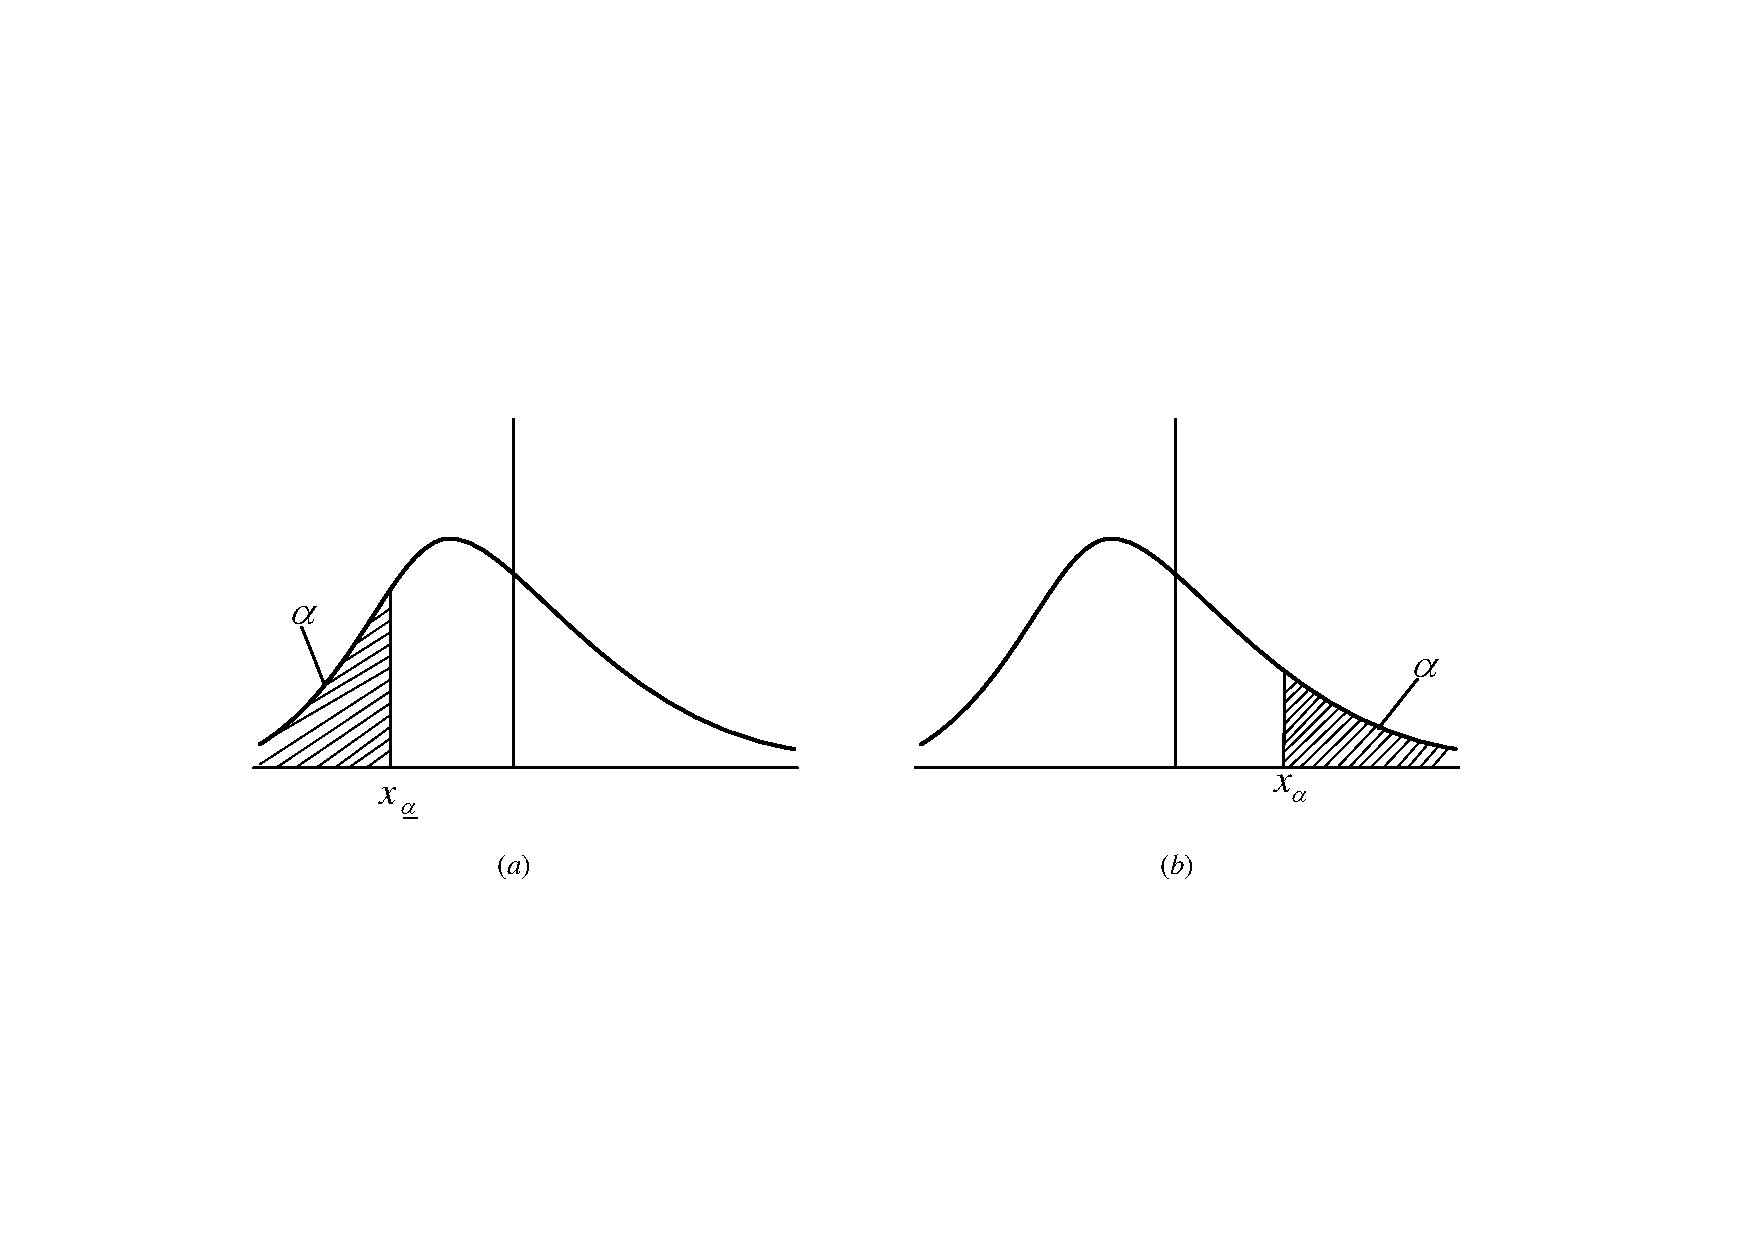
\includegraphics[width=0.8\textwidth]{4.38.pdf}
    %     \end{figure}
    
    % \begin{table}[H]\centering
    %     \begin{tabular}{c|cccccc}
    %     \hline
    %     \diagbox{$Y$}{$X$}  & 0    & 1    & 2    & 3    & 4    & 5    \\ \hline
    %     0 & 0.00 & 0.01 & 0.03 & 0.05 & 0.07 & 0.09 \\
    %     1 & 0.01 & 0.02 & 0.04 & 0.05 & 0.06 & 0.08 \\
    %     2 & 0.01 & 0.03 & 0.05 & 0.05 & 0.05 & 0.06 \\
    %     3 & 0.01 & 0.02 & 0.04 & 0.06 & 0.06 & 0.05 \\ \hline
    %     \end{tabular}
    % \end{table}


    





    \item \begin{enumerate}
        \item 在下列句子中随机地取一个单词,以$X$表示取到的单词所包含的字母个数,写出$X$的分布律,并求$E(X)$
        \begin{center}
            “THE GIRL PUT ON HER BEAUTIFUL RED HAT.”
        \end{center}
        \item 在上述句子的30个字母中随机地取一个字母,以$Y$表示取到的字母所在单词所包
        含的字母数.写出$Y$的分布律并求$E(Y)$.
        \item 一人掷骰子,如得6点则掷第2次.此时得分为$6+\mbox{第二次得到的点数}$;否则得分为
        他第一次掷得的点数,且不能再掷.求得分$X$的分布律及$E(X)$.
    \end{enumerate}


    \item 某产品的次品率为0.1,检验员每天检验4次.每次随机地取10件产品进行检验,如
    发现其中的次品数多于1,就去调整设备.以$X$表示一天中调整设备的次数,试求$E(X)$ .(设
    诸产品是否为次品是相互独立的.)



    \item 有3只球,4个盒子,盒子的编号为1,2,3,4.将球逐个独立地,随机地放入4个盒子
    中去.以$X$表示其中至少有一只球的盒子的最小号码(例如$X=3$表示第1号,第2号盒子是
    空的,第3个盒子至少有一只球),试求$E(X)$.


    \item \begin{enumerate}
        \item 设随机变量$X$的分布律为$P\left\{X=(-1)^{j+1}\dfrac{3^j}{j}\right\}=\dfrac{2}{3^j},j=1,2,\cdots$,
        说明$X$的数学期望不存在.
        \item 一盒中装有一只黑球,一只白球,作摸球游戏,规则如下:一次从盒中随机摸一只球,
        若摸到白球.则游戏结束,摸到黑球放回再放入一只黑球,然后再从盒中随机地摸一只球.试
        说明要游戏结束的摸球次数$X$的数学期望不存在.
    \end{enumerate}


    \item 设在某一规定的时间间隔里,某电气设备用于最大负荷的时间$X$(以min计)是一个
    随机变量,其概率密度为
    \vspace{-0.5cm}
    \begin{spacing}{2.0}
    $$f(x)\left\{\begin{array}[]{ll}
        
        \dfrac{1}{1500^2}x, & 0\leq x \leq 1500,\\
        -\dfrac{1}{1500^2}(x-3000), & 1500<x\leq 3000,\\
        0, &  \mbox{其他}.
    \end{array}\right.$$
    \end{spacing}
    \vspace{-0.5cm}
    求$E(X)$.


    \item \begin{enumerate}
        \item 设随机变量$X$的分布律为
        \begin{table}[H]\centering
        \begin{tabular}{c|ccc}
        $X$   & $-2$ & 0   & 2   \\ \hline
        $p_k$ & 0.4  & 0.3 & 0.3
        \end{tabular}
        \end{table}
        \vspace{-0.5cm}
        求$E(X),E(X^2),E(3X^2+5)$.
        \item 设$X\sim \pi (\lambda)$,求$E\left(\dfrac{1}{X+1}\right)$.
    \end{enumerate}


    \item \begin{enumerate}
        \item 设随机变量$X$的概率密度为
        $$f(x)=\left\{\begin{array}{ll}
            e^{-x}, & x>0\\
            0, & x\leq 0
        \end{array}
        \right.$$
        求(i)$Y=2X$,(ii)$Y=e^{-2X}$的数学期望
        \item 设随机变量$X_1,X_2,\cdots,X_n$相互独立,且都服从$(0,1)$上的均匀分布
        (i)求$U=\max\{X_1,X_2,\cdots,X_n\}$的数学期望,(ii)求$V=\min\{X_1,X_2,\cdots,X_n\}$的数学期望
    \end{enumerate}


    \item 设随机变量$(X,Y)$的分布律为
    \begin{table}[H]\centering
        \begin{tabular}{c|ccc}
        \hline
        \diagbox{$Y$}{$X$}    & 1   & 2   & 3   \\ \hline
        $-1$ & 0.2 & 0.1 & 0.0 \\
        0    & 0.1 & 0.0 & 0.3 \\
        1    & 0.1 & 0.1 & 0.1 \\ \hline
        \end{tabular}
    \end{table}
    \begin{enumerate}
        \item 求$E(X),E(Y)$.
        \item 设$Z=Y/X$,求$E(Z)$.
        \item 设$Z=(X-Y)^2$,求$E(Z)$.
    \end{enumerate}


    \item \begin{enumerate}
        \item 设随机变量$(X,Y)$的概率密度为
        $$f(x,y)=\left\{\begin{array}{ll}
            12y^2, & 0\leq y\leq x\leq 1\\
            0, & \mbox{其他}
        \end{array}\right.$$
        求$E(X),E(Y),E(XY),E(X^2+Y^2)$.
        \item 设随机变量$X,Y$的联合密度为
        \vspace{-0.5cm}
        \begin{spacing}{2.0}
        $$f(x,y)=\left\{\begin{array}{ll}
            \dfrac{1}{y}e^{-(y+x/y)}, & x>0,y>0\\
            0, & \mbox{其他}
        \end{array}\right.$$
        \end{spacing}
        \vspace{-0.5cm}
        求$E(X),E(Y),E(XY)$.
    \end{enumerate}


    \item \begin{enumerate}
        \item 设随机变量$X\sim N(0,1),Y\sim N(0,1)$且$X,Y$相互独立.求$E[X^2/(X^2+Y^2)]$.
        \item -飞机进行空投物资作业,设目标点为原点$O(0,0)$,物资着陆点为$(X,Y)$,$X,Y$相
        互独立,且设$X\sim N(0,\sigma^2),Y\sim N(0,\sigma^2)$,求原点到点$(X,Y)$间距离的数学期望.
    \end{enumerate}


    \item 一工厂生产的某种设备的寿命$X$(以年计)服从指数分布,概率密度为
    \vspace{-0.5cm}
    \begin{spacing}{2.0}
    $$f(x)=\left\{\begin{array}{ll} 
        \dfrac{1}{4}e^{-x/4}, & x>0\\
        0, & x\leq 0
    \end{array}\right.$$
    \end{spacing}
    \vspace{-0.5cm}
    工厂规定,出售的设备若在售出一年之内损坏可予以调换.若工厂售出一台设备赢利100元,
    调换一台设备厂方需花费300元.试求厂方出售一台设备净赢利的数学期望.
    

    \item 某车间生产的圆盘直径在区间$(a,b)$服从均匀分布.试求圆盘面积的数学期望.
    


    \item 设电压(以V计)$X\sim N(0,9)$.将电压施加于一检波器,其输出电压为$Y=5X^2$.求输
    出电压$Y$的均值.


    \item 设随机变量$X_1,X_2$的概率密度分别为
    $$f_1(x)=\left\{\begin{array}{ll}
        2e^{-2x}, & x>0\\
        0, & x\leq 0
    \end{array}\right.\quad
    f_2(x)=\left\{\begin{array}{ll}
        4e^{-4x}, & x>0\\
        0, & x\leq 0
    \end{array}\right.$$
    \begin{enumerate}
        \item 求$E(X_1+X_2),E(2X_1-3X_2^2)$.
        \item 又设$X_1,X_2$相互独立,求$E(X_1X_2)$.
    \end{enumerate}


    \item 将$n$只球($1\sim n$号)随机地放进$n$个盒子($1\sim n$号)中去,一个盒子装一只球.若一只
    球装入与球同号的盒子中,称为一个配对.记$X$为总的配对数,求$E(X)$.


    \item 若有$n$把看上去样子相同的钥匙.其中只有一把能打开门上的锁.用它们去试开门
    上的锁.设取到每只钥匙是等可能的.若每把钥匙试开一次后除去,试用下面两种方法求试开
    次数$X$的数学期望.
    \begin{enumerate}
        \item 写出$X$的分布律.
        \item 不写出$X$的分布律.
    \end{enumerate}
    


    \item 设$X$为随机变量,$C$是常数,证明$D(X)<E[(X-C)^2]$,对于$C\neq E(X)$.
    (由于$D(X)=E\{[X-E(X)]^2\}$,上式表明$E[(X-C)^2]$当$C=E(X)$时取到最小值.)


    \item 设随机变量$X$服从瑞利分布,其概率密度为
    \vspace{-0.5cm}
    \begin{spacing}{2.0}
    $$f(x)=\left\{\begin{array}{ll}
        \dfrac{x}{\sigma^2}e^{-\frac{x^{\scriptscriptstyle 2}}{2\sigma^{\scriptscriptstyle 2}}}, & x>0\\
        0, & x\leq 0
    \end{array}\right.$$
    \end{spacing}
    \vspace{-0.5cm}
    其中$\sigma>0$是常数,求$E(X),D(X)$.


    \item 设随机变量$X$服从$\Gamma$分布,其概率密度为
    \vspace{-0.5cm}
    \begin{spacing}{2.0}
    $$f(x)=\left\{\begin{array}{ll}
        \dfrac{1}{\beta^\alpha \Gamma(\alpha)}x^{\alpha-1}e^{-x/\beta}, & x>0\\
        0, & x\leq 0
    \end{array}\right.$$
    \end{spacing}
    \vspace{-0.5cm}
    其中$\alpha>0,\beta>0$是常数,求$E(X),D(X)$.



    \item 设随机变量$X$服从几何分布,其分布律为
    $$P\{X=k\}=p(1-p)^{k-1},\quad k=1,2,\cdots,$$
    其中$0<p<1$是常数,求$E(X),D(X)$.



    \item 设长方形的高(以m计)$X\sim U(0,2)$,已知长方形的周长(以m计)为20,求长方形面
    积$A$的数学期望和方差.


    \item \begin{enumerate}
        \item 设随机变量$X_1,X_2,X_3,X_4$相互独立,且有$E(X_i)=i,D(X_i)=5-i,i=1,2,3,4$.
        \vspace{-0.2cm}
        \begin{spacing}{2.0}
        设$Y=2X_1-X_2+3X_3-\dfrac{1}{2}X_4$.求$E(Y),D(Y)$.
        \end{spacing}
        \vspace{-0.2cm}
    \item 设随机变量$X,Y$相互独立,且$X\sim N(720,30^2),Y\sim N(640,25^2)$,求$Z_1=2X+Y,Z_2=X-Y$
    的分布,并求概率$P\{X>Y\},P\{X+Y>1400\}$.
    \end{enumerate}



    \item 五家商店联营,它们每两周售出的某种农产品的数量(以kg计)分别为$X_1,X_2,X_3,X_4,X_5$.
    已知$X_1\sim N(200,225),X_2\sim N(240,240),X_3\sim N(180,225),X_4\sim N(260,265),X_5\sim N(320,270)$,
    $X_1,X_2,X_3,X_4,X_5$相互独立.
    \begin{enumerate}
        \item 求五家商店两周的总销售量的均值和方差.
        \item 商店每隔两周进货一次,为了使新的供货到达前商店不会脱销的概率大于0.99.问
        商店的仓库应至少储存多少千克该产品?
    \end{enumerate}



    \item 卡车装运水泥,设每袋水泥重量$X$(以kg计)服从$N(50,2.5^2)$,问最多装多少袋水
    泥使总重量超过2000的概率不大于0.05.


    \item 设随机变量$X,Y$相互独立.且都服从$(0,1)$上的均匀分布.
    \begin{enumerate}
        \item 求$E(XY),E(X/Y),E[\ln (XY)],E[|Y-X|]$.
        \item 以$X,Y$为边长作一长方形,以$A,C$分别表示长方形的面积和周长,求$A$和$C$的相
        关系数.
    \end{enumerate}


    \item \begin{enumerate}
        \item 设随机变量$X_1,X_2,X_3$相互独立,且有$X_1\sim b(4,1/2),X_2\sim b(6,1/3),X_3\sim b(6,1/3)$,
        求$P\{X_1=2,X_2=2,X_3=5\},E(X_1X_2X_3),E(X_1-X_2),E(X_1-2X_2)$.
        \item 设$X,Y$是随机变量,且有$E(X)=3,E(Y)=1,D(X)=4,D(Y)=9$,令$Z=5X-Y+15$,
        分别在下列3种情况下求$E(Z)$和$D(Z)$.\\
        (i)$X,Y$相互独立,(ii)$X,Y$不相关,(iii)$X$和$Y$的相关系数为0.25.
    \end{enumerate}


    \item 下列各对随机变量$X$和$Y$,问哪几对是相互独立的?哪几对是不相关的.
    \begin{enumerate}
        \item $X\sim U(0,1),Y=X^2$
        \item $X\sim U(-1,1),Y=X^2$
        \item $X=\cos V,Y=\sin V, V\sim U(0,2\pi)$ \par
    \end{enumerate}
    若$(X,Y)$的概率密度为$f(x,y)$.
    \begin{enumerate}[resume]
        \item $$f(x,y)=\left\{\begin{array}{ll}
            x+y, & 0<x<1,0<y<1 \\
            0, & \mbox{其他}
        \end{array}\right.$$
        \item $$f(x,y)=\left\{\begin{array}{ll}
            2y, & 0<x<1,0<y<1\\
            0, & \mbox{其他}
        \end{array}\right.$$
    \end{enumerate}


    \item 设二维随机变量$(X,Y)$的概率密度为
    \vspace{-0.5cm}
    \begin{spacing}{2.0}
    $$f(x,y)=\left\{\begin{array}{ll}
        \dfrac{1}{\pi}, & x^2+y^2\leq 1\\
        0, & \mbox{其他}
    \end{array}\right.$$
    \end{spacing}
    \vspace{-0.5cm}
    试验证$X$和$Y$是不相关的,但$X$和$Y$不是相互独立的.


    \item 设随机变量$(X,Y)$的分布律为
        \begin{table}[H]\centering
        \begin{tabular}{c|ccc}
        \hline
        \diagbox{$Y$}{$X$}     & $-1$ & 0   & 1   \\ \hline
        $-1$ & 1/8  & 1/8 & 1/8 \\
        0    & 1/8  & 0   & 1/8 \\
        1    & 1/8  & 1/8 & 1/8 \\ \hline
        \end{tabular}
        \end{table}
        \vspace{-0.5cm}
    验证$X$和$Y$是不相关的,但$X$和$Y$不是相互独立的.


    \item 设$A$和$B$是试验$E$的两个事件,且$P(A)>0,P(B)>0$,并定义随机变量$X,Y$如下:
    $$X=\left\{\begin{array}{ll}
        1, & \mbox{若}A\mbox{发生}\\
        0, & \mbox{若}A\mbox{不发生}\\
    \end{array}\right.\quad
    Y=\left\{\begin{array}{ll}
        1, & \mbox{若}B\mbox{发生}\\
        0, & \mbox{若}B\mbox{不发生}\\
    \end{array}\right.\quad$$
    证明若$\rho_{XY}=0$,则$X$和$Y$必定相互独立。


    \item 设随机变量$(X,Y)$具有概率密度
    $$f(x,y)=\left\{\begin{array}{ll}
        1, & |y|<x,0<x<1\\
        0, & \mbox{其他}
    \end{array}\right.$$
    求$E(X),E(Y),\mathrm{Cov}(X,Y)$.


    \item 设随机变量$(X,Y)$具有概率密度
    \vspace{-0.5cm}
    \begin{spacing}{2.0}
    $$f(x)=\left\{\begin{array}{ll}
        \dfrac{1}{8}(x+y), & 0\leq x\leq 2,0\leq y \leq 2\\
        0, & \mbox{其他}
    \end{array}\right.$$
    \end{spacing}
    \vspace{-0.5cm}
    求$E(X),E(Y),\mathrm{Cov}(X,Y),\rho_{XY},D(X+Y)$.


    \item 设随机变量$X\sim N(\mu,\sigma^2),Y\sim N(\mu,\sigma^2)$,且设$X,Y$相互独立,试求
    $Z_1=\alpha X+\beta Y$和$Z_2=\alpha X-\beta Y$的相关系数(其中$\alpha,\beta$是不为零的常数).


    \item \begin{enumerate}
        \item 设随机变量$W=(aX+3Y)^2,E(X)=E(Y)=0,D(X)=4,D(Y)=16,\rho_{XY}=-0.5$.求常数$a$
        使$E(W)$为最小,并求$E(W)$的最小值。
        \item 设随机变量$(X,Y)$服从二维正态分布,且有$D(X)=\sigma_X^2,D(Y)=\sigma_Y^2$.证明当$a^2=\sigma^2_X/\sigma^2_Y$
        时,随机变量$W=X-aY$与$V=X+aY$相互独立。
    \end{enumerate}


    \item 设随机变量$(X,Y)$服从二维正态分布,且$X\sim N(0,3),Y\sim N(0,4)$,相关系数$\rho_{XY}=-1/4$,
    试写出$X$和$Y$的联合概率密度.
    
    
    \item 已知正常男性成人血液中,每一亳升白细胞数平均是7300,均方差是700.利用切比
    雪夫不等式估计每毫升含白细胞数在$5200\sim 9400$之间的概率$p$.
    
    
    \item 对于两个随机变量$V,W$,若$E(V^2),E(W^2)$存在,证明
    $$[E(VW)]^2\leq E(V^2)E(W^2)$$
    这一不等式称为柯西-施瓦茨不等式
    \par 提示:考虑实变量$t$的函数
    $$q(t)=E[(V+tW)^2]=E(V^2)+2tE(VW)+t^2E(W^2)$$




  

\end{enumerate}
\end{document}